% !TEX TS-program = XeLaTeX
% use the following command:
% all document files must be coded in UTF-8
\documentclass[english]{textolivre}
% build HTML with: make4ht -e build.lua -c textolivre.cfg -x -u article "fn-in,svg,pic-align"

\journalname{Texto Livre}
\thevolume{18}
%\thenumber{1} % old template
\theyear{2025}
\receiveddate{\DTMdisplaydate{2025}{1}{4}{-1}} % YYYY MM DD
\accepteddate{\DTMdisplaydate{2025}{4}{16}{-1}}
\publisheddate{\DTMdisplaydate{2025}{8}{8}{-1}}
\corrauthor{Oksana Chugai}
\articledoi{10.1590/1983-3652.2025.56839}
%\articleid{NNNN} % if the article ID is not the last 5 numbers of its DOI, provide it using \articleid{} commmand 
% list of available sesscions in the journal: articles, dossier, reports, essays, reviews, interviews, editorial
\articlesessionname{articles}
\runningauthor{Chugai, Lytovchenko and Synekop} 
%\editorname{Leonardo Araújo} % old template
\sectioneditorname{Daniervelin Pereira}
\layouteditorname{Saula Cecília}

\title{University teachers’ perceptions, experiences and implications for using ChatGPT in ESL}
\othertitle{Percepções, experiências e implicações de professores universitários para o uso do ChatGPT em ESL}
% if there is a third language title, add here:
%\othertitle{Artikelvorlage zur Einreichung beim Texto Livre Journal}

\author[1]{Oksana Chugai~\orcid{0000-0002-2118-8255}\thanks{Email: \href{mailto:OChugai@meta.ua}{OChugai@meta.ua}}}
\author[1]{Iryna Lytovchenko~\orcid{0000-0002-8578-3985}\thanks{Email: \href{mailto:irinalytovch@gmail.com}{irinalytovch@gmail.com}}}
\author[1]{Oksana Synekop~\orcid{0000-0001-6191-6264}\thanks{Email: \href{mailto:oksana.synekop@gmail.com}{oksana.synekop@gmail.com}}}
\affil[1]{National Technical University of Ukraine ``Igor Sikorsky Kyiv Polytechnic Institute", Department of English for Engineering Nº 2, Kyiv, Ukraine.}


\addbibresource{article.bib}
% use biber instead of bibtex
% $ biber article

% used to create dummy text for the template file
\definecolor{dark-gray}{gray}{0.35} % color used to display dummy texts
\usepackage{lipsum}
\SetLipsumParListSurrounders{\colorlet{oldcolor}{.}\color{dark-gray}}{\color{oldcolor}}

% used here only to provide the XeLaTeX and BibTeX logos
\usepackage{hologo}

% if you use multirows in a table, include the multirow package
\usepackage{multirow}

% provides sidewaysfigure environment
\usepackage{rotating}

% CUSTOM EPIGRAPH - BEGIN 
%%% https://tex.stackexchange.com/questions/193178/specific-epigraph-style
\usepackage{epigraph}
\renewcommand\textflush{flushright}
\makeatletter
\newlength\epitextskip
\pretocmd{\@epitext}{\em}{}{}
\apptocmd{\@epitext}{\em}{}{}
\patchcmd{\epigraph}{\@epitext{#1}\\}{\@epitext{#1}\\[\epitextskip]}{}{}
\makeatother
\setlength\epigraphrule{0pt}
\setlength\epitextskip{0.5ex}
\setlength\epigraphwidth{.7\textwidth}
% CUSTOM EPIGRAPH - END

% to use IPA symbols in unicode add
%\usepackage{fontspec}
%\newfontfamily\ipafont{CMU Serif}
%\newcommand{\ipa}[1]{{\ipafont #1}}
% and in the text you may use the \ipa{...} command passing the symbols in unicode

% LANGUAGE - BEGIN
% ARABIC
% for languages that use special fonts, you must provide the typeface that will be used
% \setotherlanguage{arabic}
% \newfontfamily\arabicfont[Script=Arabic]{Amiri}
% \newfontfamily\arabicfontsf[Script=Arabic]{Amiri}
% \newfontfamily\arabicfonttt[Script=Arabic]{Amiri}
%
% in the article, to add arabic text use: \textlang{arabic}{ ... }
%
% RUSSIAN
% for russian text we also need to define fonts with support for Cyrillic script
% \usepackage{fontspec}
% \setotherlanguage{russian}
% \newfontfamily\cyrillicfont{Times New Roman}
% \newfontfamily\cyrillicfontsf{Times New Roman}[Script=Cyrillic]
% \newfontfamily\cyrillicfonttt{Times New Roman}[Script=Cyrillic]
%
% in the text use \begin{russian} ... \end{russian}
% LANGUAGE - END

% EMOJIS - BEGIN
% to use emoticons in your manuscript
% https://stackoverflow.com/questions/190145/how-to-insert-emoticons-in-latex/57076064
% using font Symbola, which has full support
% the font may be downloaded at:
% https://dn-works.com/ufas/
% add to preamble:
% \newfontfamily\Symbola{Symbola}
% in the text use:
% {\Symbola }
% EMOJIS - END

% LABEL REFERENCE TO DESCRIPTIVE LIST - BEGIN
% reference itens in a descriptive list using their labels instead of numbers
% insert the code below in the preambule:
%\makeatletter
%\let\orgdescriptionlabel\descriptionlabel
%\renewcommand*{\descriptionlabel}[1]{%
%  \let\orglabel\label
%  \let\label\@gobble
%  \phantomsection
%  \edef\@currentlabel{#1\unskip}%
%  \let\label\orglabel
%  \orgdescriptionlabel{#1}%
%}
%\makeatother
%
% in your document, use as illustraded here:
%\begin{description}
%  \item[first\label{itm1}] this is only an example;
%  % ...  add more items
%\end{description}
% LABEL REFERENCE TO DESCRIPTIVE LIST - END


% add line numbers for submission
%\usepackage{lineno}
%\linenumbers

\begin{document}
\maketitle

\begin{polyabstract}
\begin{abstract}
Artificial Intelligence (AI) has become an inseparable part of higher education, affecting the various educational environments. Teachers play a vital role in adopting new educational tools, including AI technology. However, the use of AI, ChatGPT in particular, in language learning remains under-investigated. This study aims to explore English as a Second Language (ESL) teachers’ perceptions of using ChatGPT, their hands-on experiences and implications for future research. We used a mixed research design to collect quantitative and qualitative data based on a five-point Likert scale. Key findings indicate that nearly sixty percent of ESL teachers were satisfied with ChatGPT’s assistance, and half thought it positively influenced their performance as ESL teachers. ChatGPT was easy to use for two-thirds of respondents. However, more than half of ESL teachers described challenges like faulty or irrelevant information that needed checking, low-quality responses and ethical issues. Interestingly, the majority of ESL teachers would recommend implementing ChatGPT into teaching. Whereas it saves time for teachers doing routine tasks, providing immediate feedback and generating ideas, it is evident that ESL teachers need more training in developing AI literacy. This exploratory study requires further research, which could investigate perceptions of educators with wider levels of expertise and areas of professional interest.

\keywords{English as a Second Language (ESL) \sep Artificial intelligence (AI) \sep ChatGPT \sep University teachers \sep Professional development}
\end{abstract}

\begin{portuguese}
\begin{abstract}
A Inteligência Artificial (IA) tornou-se uma parte inseparável do ensino superior, afetando os diversos ambientes educacionais. Os professores desempenham um papel vital na adoção de novas ferramentas educacionais, incluindo a tecnologia de IA. No entanto, o uso de IA, em particular o ChatGPT, na aprendizagem de línguas continua pouco investigado. Este estudo tem como objetivo explorar as percepções dos professores de Inglês como Segunda Língua (ESL, na sigla em inglês) sobre o uso do ChatGPT, suas experiências práticas e implicações para pesquisas futuras. Utilizamos um desenho de pesquisa misto para coletar dados quantitativos e qualitativos com base em uma escala Likert de cinco pontos. As principais conclusões indicam que quase sessenta por cento dos professores de ESL ficaram satisfeitos com a assistência do ChatGPT, e metade deles considerou que isso influenciou positivamente o seu desempenho como professores de ESL. O ChatGPT foi fácil de usar para dois terços dos entrevistados. No entanto, mais de metade dos professores de ESL descreveram desafios como informações defeituosas ou irrelevantes que precisavam de ser verificadas, respostas de baixa qualidade e questões éticas. Curiosamente, a maioria dos professores de ESL recomendaria a implementação do ChatGPT no ensino. Embora economize tempo para os professores realizarem tarefas rotineiras, fornecendo feedback imediato e gerando ideias, é evidente que os professores de ESL precisam de mais formação no desenvolvimento da literacia em IA. Este estudo exploratório requer mais pesquisas que possam investigar as percepções de educadores com níveis mais amplos de especialização e áreas de interesse profissional.

\keywords{Inglês como Segunda Língua (ESL) \sep Inteligência Artificial (IA) \sep ChatGPT \sep Professores universitários \sep Desenvolvimento profissional} 
\end{abstract}
\end{portuguese}
% if there is another abstract, insert it here using the same scheme
\end{polyabstract}

\section{Introduction}
The traditional educational environment welcomes innovative digital technologies, which have become an inseparable part of teachers’ and students’ lives. However, concerns that Artificial Intelligence (AI) affects education in many aspects and has disruptive impacts are expressed in many studies \cites[p. 21]{bereczki2021}{hie2023}[p. 249]{sumakul2022}. The current state of English as a Second Language (ESL) education is characterized by a fusion of conventional teaching methods and emerging technological solutions. According to recent research based on bibliometric analysis, the number of papers focusing on AI has increased significantly. However, AI applications in ESL remain under-investigated \cite[p. 112]{huang2023}. There is also a lack of research on AI focusing on university teachers’ perspectives \cites[p. 1]{schroder2023}[p. 132]{synekop2024}[p. 16]{zawacki-richter2019}. Despite the need for optimization of human teachers’ workload, the evidence for collaboration between conversational AIs and ESL teachers is limited \cite[p. 48]{ji2022}. Therefore, the integration of AI, ChatGPT in particular, which is called ``a state-of-the-art language model", needs an in-depth analysis of its implications in ESL classrooms \cites[p. 542]{holmes2022}[p. 97]{iqbal2023}. One approach to conducting such analysis is to explore ESL teachers’ perceptions towards the use of AI, their hands-on experiences and implications for future research.

Understanding university teachers’ perceptions and experiences of using ChatGPT in ESL classrooms is crucial for several reasons. First of all, teachers play a vital role in promoting holistic students’ development and enhancing learning outcomes \cite[p. 7591]{mavropoulou2023}. The importance of investigating teachers’ perceptions is based on their ability to utilize technological advances through classroom instruction, thus being evidence of their social validity \cite{wilson2021}. Secondly, exploring teachers’ perceptions and experiences helps in evaluating the effectiveness of ChatGPT in ESL instruction and provides a deeper understanding of teaching practice, which is vital for the adoption of new educational tools. Furthermore, such research highlights potential challenges and benefits associated with the use of ChatGPT in ESL classrooms. Learning more about teachers’ perceptions is vitally important to reveal barriers, meet teachers’ needs regarding the use of technological advances in classrooms, and design professional development programs \cites[p. 67]{cope2002}[p. 309]{ottenbreit-leftwich2018}. Having valuable insights into the integration of AI technology in language education allows ESL teachers to make informed decisions about incorporating such tools into their teaching practices. Based on the analysis of studies, it becomes evident that teachers play a vital role in introducing AI in education. At the same time, there is a lack of scientific research on university teachers’ perceptions and experiences related to using ChatGPT in ESL.

The article aims to explore ESL teachers’ perceptions, experiences and implications of using ChatGPT. To achieve the aim, the following research questions should be answered:

\medskip
\begin{itemize}
    \item What are the characteristics of the participants of the research?
    \item What is university teachers’ usage of ChatGPT in terms of frequency, purposes and level of satisfaction?
    \item What is ChatGPT’s impact on teaching practice?
    \item How user-friendly is ChatGPT for university teachers?
    \item What are the responders’ recommendations on using ChatGPT in ESL?
\end{itemize}
\medskip

The exploration of university teachers’ perceptions and experiences of ChatGPT in ESL classrooms will contribute to existing literature. It may be transferrable to other educational environments in terms of informing decision-making, evaluating effectiveness and addressing challenges, thus facilitating the integration of AI into language education.

\section{Literature Review}
To employ ChatGPT as a resource to enhance engagement and adaptability in language learning, it is important to be aware of its characteristics, advantages and disadvantages. One of the significant advantages of incorporating ChatGPT into ESL teaching is its capacity to offer personalized and interactive language practice. Its extensive language database facilitates tailored exercises, allowing educators to cater to individual student needs and preferences. Furthermore, ChatGPT serves as a valuable tool for generating authentic and contextually relevant language content, enabling ESL teachers to create exercises and simulations that mirror real-world communication. The main advantages of using ChatGPT for learners are in creating meaningful content, supporting production, and providing feedback aimed at language fluency development. Concerning teachers, it helps with designing lessons, creating teaching materials, and providing feedback to develop their professional skills \cite[p. 3]{meniado2023}.

However, educators face challenges when integrating ChatGPT in ESL classrooms. The most acute drawbacks of using AI in education are as follows: ethics, efficacy and impact, AIED colonialism, and commercialization \cite[p. 558]{holmes2022}. Another concern is its occasional lack of contextual and cultural authenticity. ESL educators must exercise caution, as relying solely on ChatGPT may result in responses that are not natural in a language learning environment. The potential for overreliance on technology is also disturbing, as it may lead to diminishing the vital role of human interaction in the ESL learning process. It is crucial to ensure that ChatGPT complements the human element in language education. Teachers should explore their students’ level of AI literacy to meet their needs. The previous research findings indicated students’ concerns about the potential risks of AI technologies \cite[p. 14]{chan2023}. Drawbacks also include erroneous and general responses, academic misconduct, detrimental effects on skills development, biased information, limitation of access and unemployment of teachers in the future \cite[p. 3]{meniado2023}. On the one hand, educators have an opportunity to use the latest technological advances; on the other, being AI literate, they are expected to be responsible for applying it in education \cite[p. 543]{holmes2022}.

The multiple case study on teachers’ beliefs and experiences related to the integration of creativity into technological learning environments revealed stereotypical views and suggested introducing curricular timeframes \cite[p. 21]{bereczki2021}. It was pointed out in recent research that there are three types of teachers’ beliefs: epistemic, pedagogical, and the ones about the use of technology in education, which are closely interrelated \cites[p. 245]{deng2014}[p. 20]{ding2019}. It was found that it was important to consider teachers’ technological and pedagogical knowledge before integrating AI in ESL classes, as there is an overall alignment between ESL teachers’ pedagogical beliefs and the integration of technology into their lessons \cites[p. 20]{ding2019}[p. 33]{sumakul2023}[p. 249]{sumakul2022}. Other empirical studies \cite{ertmer2005} examined four dimensions of teachers’ uses of technological advances: ``self-efficacy, attitudes, pedagogical beliefs, and openness to change" \cite[p. 309]{ottenbreit-leftwich2018}. Another dimension is risk-taking, which is a coping strategy for experimenting with new tools \cite[p. 1351]{howard2016}. However, risk-taking means readiness to change, therefore, these terms (``risk-taking" and ``openness to change") may be used interchangeably. Considering AIs as teachers’ assistants, the roles of human teachers are changing – they have to develop new skills labeled as ACE (analytical, creative, evaluative), which should be supported by teacher professional development programs \cite[p. 42]{sumakul2019}.


\section{Materials and Methods}
The basis of the study was a mixed research design to collect quantitative and qualitative data through an online survey. An anonymous questionnaire was developed specifically for ESL university teachers to define the perceptions, experiences, and implications of using ChatGPT in ESL. The collected data was analyzed, interpreted, and summarised.

The respondents were ESL university teachers ($N=34$) from various educational establishments in Ukraine to ensure a representative sample of perspectives related to the teaching of English as a second language using ChatGPT in the country. The diversity increases the credibility and richness of the data collected. Ultimately, it contributes to a more nuanced understanding of the use of tools such as ChatGPT in language teaching. The respondents signed an informed consent, and their participation in the research in December 2023 was voluntary and anonymous.

An online survey was the main tool in our research. The survey covered five sections on demographic information (4 questions), ChatGPT usage (3 questions), impact on teaching (2 questions), user experience (2 questions) and future recommendations for exploiting ChatGPT in ESL (2 questions). The survey included closed-ended questions to gather quantitative data, allowing statistical analysis of trends and patterns, and open-ended questions to elicit qualitative feedback, enriching understanding of individual experiences and perspectives. The quantitative research method was used to process the data. To show what most respondents chose and how strongly they agreed with each other, the median (Mdn) and Inter-Quartile Range (IQR) on a five-point Likert scale were calculated, in case it was possible. The qualitative research method was applied for processing written responses.

Data was collected through the Google Forms application shared with university teachers through social networking sites and emails. Using Google Forms not only streamlined the data collection process but also allowed participants to respond when it suited them, thereby increasing the overall response rate.

\section{Results and Discussion}

\subsection{Demographic aspects}
Demographic aspects are important as they reveal the diversity within the respondents, aiding in a better understanding of patterns influenced by factors like age, gender and experience. The current study showed that the age range of the participants varied from 25 to 55 plus (Figure \ref{fig-1}).

%---- CÓDIGO DA FIGURA 1 ----%
\begin{figure}[h!]
    \centering
    \begin{minipage}{0.65\linewidth}
    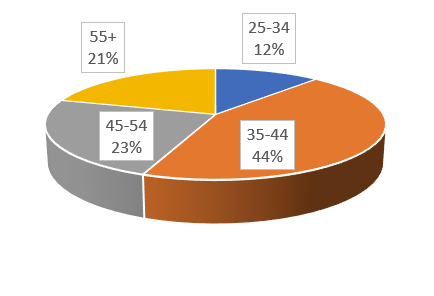
\includegraphics[width=\linewidth]{Imagens/Figure1.png}
    \caption{Respondents’s age.}
    \label{fig-1}
    \source{Own elaboration (2024).}
    \end{minipage}
\end{figure}

Nearly half of the respondents were between 35 and 44 years old, more than twenty percent in the age range from 45 to 54, and the same percentage were aged 55 plus. A bit more than half of the participants had working experience of at least twenty-one years, and a third had between eleven and twenty years of teaching experience (Figure \ref{fig-2}).

%---- CÓDIGO DA FIGURA 2 ----%
\begin{figure}[h!]
    \centering
    \begin{minipage}{0.65\linewidth}
    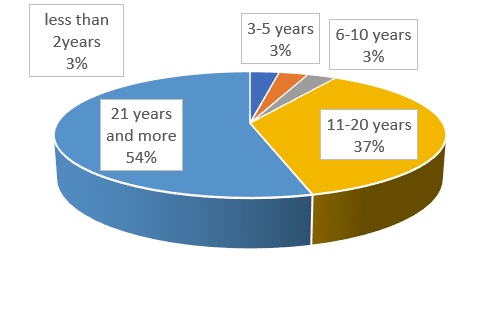
\includegraphics[width=\linewidth]{Imagens/Figure2.png}
    \caption{Respondents’ working experience.}
    \label{fig-2}
    \source{Own elaboration (2024).}
    \end{minipage}
\end{figure}

All respondents were university teachers from various educational establishments in Ukraine. The majority of them were women (Figure \ref{fig-3}).

%---- CÓDIGO DA FIGURA 3 ----%
\begin{figure}[h!]
    \centering
    \begin{minipage}{0.7\linewidth}
    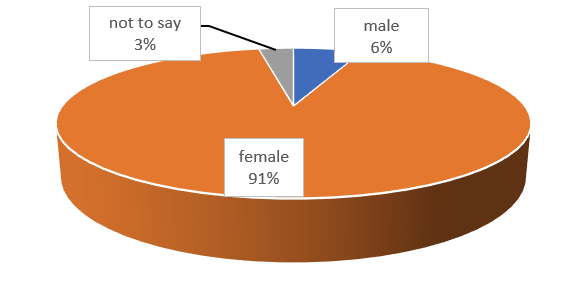
\includegraphics[width=\linewidth]{Imagens/Figure3.png}
    \caption{Respondents’ gender.}
    \label{fig-3}
    \source{Own elaboration (2024).}
    \end{minipage}
\end{figure}

The obtained data could be explained by the increasing percentage of senior citizens in Ukraine, which gradually led to greater numbers of middle-aged teachers. On the other hand, the low prestige of teachers as such resulted in a decreasing number of young educators \cite[p. 5]{ivanishchenko2020}. Considering gender, eighty-four percent of teachers in Ukraine were women, which was higher than the international average, sixty-one percent \cite{lisova2018}. Another research based on TALIS (Teaching and Learning International Survey) confirmed the predominance of women over men in the teaching profession in Ukraine \cite[p. 10]{ivanishchenko2020}. Such gender asymmetry could be a result of the phenomenon of the ``concealed higher school curriculum" which generated gender stereotypes \cite[p. 662]{petruchenia2014}. Eventually, the war in Ukraine led to casualties and emigration, which resulted in a shrinking labor force and rapid aging \cite[p. 245]{perelli-harris2023}. At the same time, females constituted 65\% in another study as well, with a considerable number of respondents older than 30 years with experience in teaching for more than 10 years \cite[p. 14]{nguyen2023}. To sum up, middle-aged women, university lecturers in Ukraine, with experience in teaching English for about twenty years or more, prevailed among respondents in our research.

\subsection{Frequency of ChatGPT usage}
Understanding the frequency of ChatGPT usage is crucial for insights into ESL teachers’ engagement, enabling a conclusion about the overall user experience. According to the results of our research, about forty percent of respondents used ChatGPT occasionally (Figure \ref{fig-4}).

%---- CÓDIGO DA FIGURA 4 ----%
\begin{figure}[h!]
    \centering
    \begin{minipage}{0.65\linewidth}
    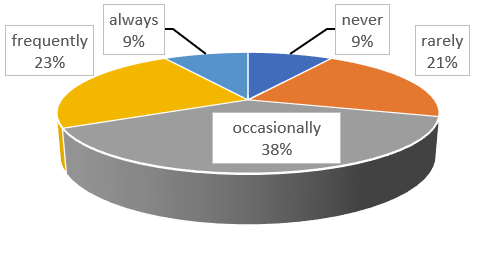
\includegraphics[width=\linewidth]{Imagens/Figure4.png}
    \caption{Frequency of ChatGPT usage.}
    \label{fig-4}
    \source{Own elaboration (2024).}
    \end{minipage}
\end{figure}

Approximately the same number of respondents used ChatGPT either frequently (23\%) or rarely (21\%). Remarkably, nine percent of university teachers never used ChatGPT. Considering a measure of the central tendency, the most probable answer for using ChatGPT by university teachers was ``occasionally" (Mdn=3). Meanwhile, a measure of spread showed that the responses were not scattered across the range (IQR=2) (Table \ref{tab-1}).

%---- CÓDIGO DA TABELA 1 ----%
\begin{table}[h!]
\centering
\caption{University teachers’ frequency of ChatGPT usage.}\label{tab-1}
\begin{tabularx}{\textwidth}{@{}Xccccccc@{}}
\toprule
Question & Never & Rarely & Occasionally & Frequently & Always & Mdn & IQR \\
\midrule
How frequently do you use ChatGPT for academic purposes? & 3 (9\%) & 7 (21\%) & 13 (38\%) & 8 (23\%) & 3 (9\%) & 3 & 2 \\
\bottomrule
\end{tabularx}
\source{Own elaboration (2024).}
\end{table}

The findings of previous research showed that, experiencing teaching online during the pandemic, teachers planned their lessons more carefully, taking into consideration the individual characteristics of the learners and possible technical problems they could experience \cites[p. 9]{kohnke2023}[p. 20]{westerlund2023}. The findings of other studies showed that teachers used ChatGPT occasionally, and some respondents just had several attempts to try it \cites[p. 107]{iqbal2023}[p. 136]{synekop2024}. Similarly, research on higher education teachers using open educational resources showed that they did not use AI \cite[p. 14]{schroder2023}. In contrast, the majority of participants in the previous study often used ChatGPT, and a quarter of teachers did so occasionally \cite[p. 15]{nguyen2023}. Understanding the purposes of ChatGPT usage by ESL teachers reveals their needs, expectations, and their awareness of its capabilities. Based on the analysis of the responses in the current research, we conclude that ESL teachers often used ChatGPT to prepare writing assignments for their students (49\%) (Figure \ref{fig-5}).

%---- CÓDIGO DA FIGURA 5 ----%
\begin{figure}[h!]
    \centering
    \begin{minipage}{0.70\linewidth}
    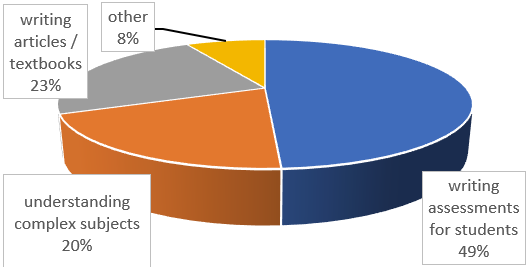
\includegraphics[width=\linewidth]{Imagens/Figure5.png}
    \caption{Purposes of ChatGPT usage.}
    \label{fig-5}
    \source{Own elaboration (2024).}
    \end{minipage}
\end{figure}

Respondents also turned to ChatGPT assistance when they had to write articles and textbooks (23\%) or needed help with understanding complex concepts (20\%). In some cases, respondents wanted to improve their writing skills, design assessment plans, or check writing assignments (8\%). It is important to know that respondents usually had several purposes for using ChatGPT. These findings align with other studies that indicated teachers’ positive attitude towards using ChatGPT in writing classes, as well as in their research and academic writing \cites[p. 106]{iqbal2023}[p. 39]{nguyen2023}. A study focused on applying AI by French language teachers proved that AI provides a valuable service by creating learning materials \cite[p. 7591]{mavropoulou2023}. Previous studies also revealed the effectiveness of using ChatGPT in ESL writing classes, but at the same time, the ``threats to academic honesty and educational equity" as well, which led to the necessity of reconsidering academic dishonesty and regulatory policy \cite{yan2023}. Another research revealed a more sophisticated approach to utilizing ChatGPT – besides writing assistance, ``personalized learning and intelligent tutoring systems" were also in high demand \cite[p. 112]{huang2023}.

Our findings showed that ESL teachers in our research did not specify or were possibly not aware of some other ways of using ChatGPT, like interactive conversations, pronunciation practice, and exposure to different cultures, dialects and styles of English \cite[p. 3]{kostka2023}. Some practical ways of applying ChatGPT in an ESL class could be presenting definitions of new words and expressions, their usage in various contexts and additional grammatical information; generating grammar or vocabulary quizzes; writing dialogues or stories at different language proficiency levels and in various genres; answering questions and responding in any language, be it a target or mother tongue \cite[p. 539-544]{kohnke2023}.

Exploring ESL teachers’ satisfaction with ChatGPT is vital for learning more about educators’ needs for its integration into language teaching. It provides a valuable tool for professional development and skill enhancement, and fosters a supportive community sharing experiences and best practices. According to the results of the research, nearly sixty percent of ESL teachers claimed that they were satisfied with ChatGPT’s assistance (Figure \ref{fig-6}).

%---- CÓDIGO DA FIGURA 6 ----%
\begin{figure}[h!]
    \centering
    \begin{minipage}{0.70\linewidth}
    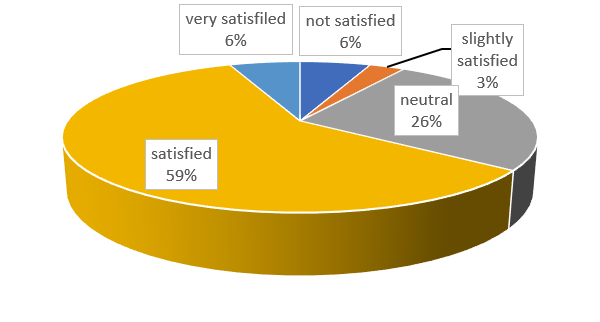
\includegraphics[width=\linewidth]{Imagens/Figure6.png}
    \caption{Respondents’ satisfaction with ChatGPT’s assistance.}
    \label{fig-6}
    \source{Own elaboration (2024).}
    \end{minipage}
\end{figure}

%---- CÓDIGO DA TABELA 2 ----%
\setlength{\tabcolsep}{3pt} % reduz espaço interno das células
\begin{table}[h!]
\centering
\caption{University teachers’ satisfaction with ChatGPT’s assistance.}\label{tab-2}
\begin{tabular}{@{}p{3cm}
                >{\centering\arraybackslash}p{1.9cm}
                >{\centering\arraybackslash}p{1.9cm}
                >{\centering\arraybackslash}p{1.4cm}
                >{\centering\arraybackslash}p{1.6cm}
                >{\centering\arraybackslash}p{1.9cm}
                >{\centering\arraybackslash}p{0.65cm}
                >{\centering\arraybackslash}p{0.65cm}@{}}
\toprule
Question & Not satisfied\newline at all & Slightly\newline satisfied & Neutral & Satisfied & Very\newline satisfied & Mdn & IQR \\
\midrule
How satisfied are you with ChatGPT’s assistance? & 2 (6\%) & 1 (3\%) & 9 (26\%) & 20 (59\%) & 2 (6\%) & 4 & 1 \\
\bottomrule
\end{tabular}
\source{Own elaboration (2024).}
\end{table}


The central tendency was to choose ``satisfied" (Mdn=4); respondents mostly agreed with each other (IQR=1) (Table \ref{tab-2}). Our findings align with the results of another study, which showed that 60\% of teachers were positive about ChatGPT’s assistance with designing learning materials \cite[p. 16]{nguyen2023}. The findings of the study on the impact of AI on learning English in Saudi Arabia also showed that teachers were mostly positive about using Artificial Intelligence in their ESL classes \cite[p. 36]{aljohani2021}. ESL teachers’ perceptions in another study were also positive: the participants agreed that ``AI could help teachers teach and students learn" \cite[p. 232]{sumakul2022}. Meanwhile, a quarter of respondents in our study were neither positive nor negative. A prior research on teachers’ attitudes towards ChatGPT indicated the reason for their negative attitude, which was the possibility for students to cheat and become lazy \cite[p. 102]{iqbal2023}.

\subsection{ChatGPT’s impact on ESL teaching}
Learning more about ChatGPT’s impact on ESL teaching is vital to creating engaging language learning environments. Regarding ChatGPT’s influence on improvements in ESL teachers’ practice, the findings of our research showed that sixty-five percent of respondents were positive, choosing ``moderately", ``very much" and ``extremely" (Figure \ref{fig-7}).

%---- CÓDIGO DA FIGURA 7 ----%
\begin{figure}[h!]
    \centering
    \begin{minipage}{0.70\linewidth}
    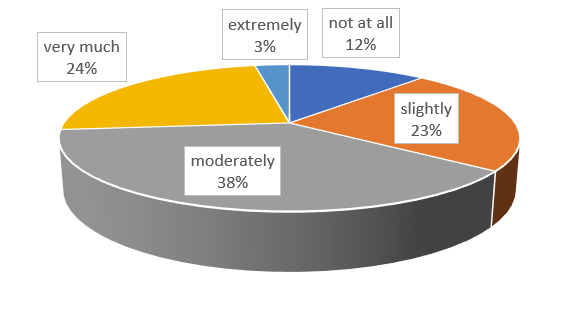
\includegraphics[width=\linewidth]{Imagens/Figure7.png}
    \caption{ChatGPT assists in improving teaching practice.}
    \label{fig-7}
    \source{Own elaboration (2024).}
    \end{minipage}
\end{figure}

The central tendency indicated ``moderately" (Mdn=3), and the participants tended to agree with each other (IQR=1.8) (Table \ref{tab-3}).

%---- CÓDIGO DA TABELA 3 ----%
\begin{table}[h!]
\centering
\caption{ChatGPT’s impact on teaching practice.}\label{tab-3}
\begin{tabularx}{\textwidth}{@{}Xccccc cc@{}}
\toprule
Question & Not at all & Slightly & Moderately & Very much & Extremely & Mdn & IQR \\
\midrule
To what extent has ChatGPT improved your teaching practice? & 4 (12\%) & 8 (23\%) & 13 (38\%) & 8 (24\%) & 1 (3\%) & 3 & 1.8 \\
\bottomrule
\end{tabularx}
\source{Own elaboration (2024).}
\end{table}


Such findings are in sharp contrast with previous research, which showed that the majority of teachers thought ChatGPT was useless, disruptive, and could result in cheating and plagiarism \cite[p. 103]{iqbal2023}. As evident from the results, half of the participants thought that using ChatGPT positively influenced their performance as teachers (their choices were ``agree" and ``strongly agree") (Figure \ref{fig-8}).

%---- CÓDIGO DA FIGURA 8 ----%
\begin{figure}[h!]
    \centering
    \begin{minipage}{0.65\linewidth}
    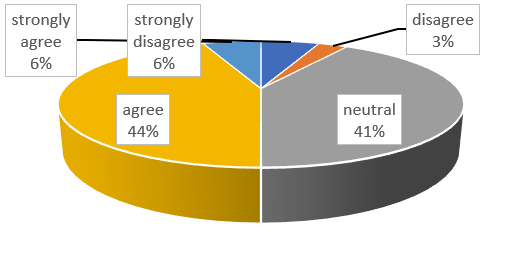
\includegraphics[width=\linewidth]{Imagens/Figure8.png}
    \caption{ChatGPT’s influence on teachers’ performance.}\label{tab-4}
    \label{fig-8}
    \source{Own elaboration (2024).}
    \end{minipage}
\end{figure}

%---- CÓDIGO DA TABELA 4 ----%
\begin{table}[h!]
\centering
\caption{ChatGPT’s impact on teachers’ performance.}
\begin{tabularx}{\textwidth}{@{}Xccccc cc@{}}
\toprule
Question & SD & D & N & A & SA & Mdn & IQR \\
\midrule
Has using ChatGPT positively influenced your performance? & 2 (6\%) & 1 (3\%) & 14 (41\%) & 15 (44\%) & 2 (6\%) & 3.5 & 1 \\
\bottomrule
\end{tabularx}
\source{Own elaboration (2024).}
\end{table}

However, the central tendency was between those who chose “neutral” and those who opted for ``agree" (Mdn=3.5), and the responses were clustered together (IQR=1) (Table \ref{tab-4}). According to another research, some educators found ChatGPT useful in providing immediate feedback for students, which saved time for teachers to be engaged in more creative activities \cite[p. 102]{iqbal2023}.

\subsection{ChatGPT user experience of university teachers}
Learning more about the user experience of university teachers with ChatGPT is instrumental for the educational community. Regarding simplicity, it was easy or very easy to use ChatGPT for two-thirds of respondents in our research, while a quarter of ESL teachers were neither positive nor negative (Figure \ref{fig-9}).

%---- CÓDIGO DA FIGURA 9 ----%
\begin{figure}[h!]
    \centering
    \begin{minipage}{0.65\linewidth}
    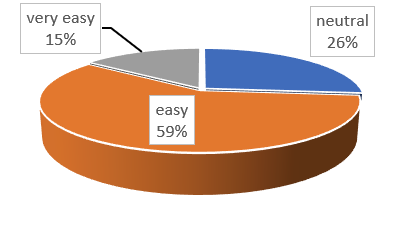
\includegraphics[width=\linewidth]{Imagens/Figure9.png}
    \caption{ChatGPT’s influence on teachers’ performance.}
    \label{fig-9}
    \source{Own elaboration (2024).}
    \end{minipage}
\end{figure}

The central tendency indicated that it was easy to use ChatGPT (Mdn=4), and the participants agreed with each other (IQR=0.8) (Table \ref{tab-5}).

%---- CÓDIGO DA TABELA 5 ----%
\begin{table}[h!]
\centering
\caption{How user-friendly ChatGPT is for university teachers.}\label{tab-5}
\begin{tabularx}{\textwidth}{@{}Xccccc cc@{}}
\toprule
Question & Very difficult & Difficult & Neutral & Easy & Very easy & Mdn & IQR \\
\midrule
How user-friendly do you find ChatGPT for your academic needs? & 0 & 0 & 9 (26\%) & 20 (59\%) & 5 (15\%) & 4 & 0.8 \\
\bottomrule
\end{tabularx}
\source{Own elaboration (2024).}
\end{table}


According to previous research, teachers confessed that they were not ready to use ChatGPT in their classrooms as they lacked the necessary skills and, therefore, needed additional training and support \cite[p. 104]{iqbal2023}. Participants of a similar research rated their experience as moderately challenging, reporting technical issues \cite[p. 16]{nguyen2023}. As far as there is a need for integration of technological tools in education, there is an urgent necessity to educate digitally competent teachers \cite{instefjord2017}.

Collecting data about the challenges and limitations faced by ESL teachers using ChatGPT is instrumental in facilitating ongoing improvement. In our research, a bit more than half of the respondents (53\%) described challenges or limitations they experienced using ChatGPT; others either did not use it or found no faults. The participants in our study complained that information generated by ChatGPT ``needs additional verification and critical revision", which means ``double work" for users as ``it makes mistakes", ``information is often irrelevant, needs considerable reviewing, checking, and editing". Most importantly, the accuracy of ChatGPT responses is even more significant as they look quite plausible, which may be confusing for learners \cite[p. 545]{kohnke2023}.

The quality of ChatGPT responses was also not satisfying for ESL teachers who stated that ``sometimes GPT doesn’t get what I want", ``it provides long answers", ``tests are quite complex, for example, two questions in one", etc. Other drawbacks were a lack of citation and technical features. Indeed, one of the main drawbacks of using ChatGPT is related to ethical use, as there are no citations or sources of the generated information, and therefore, it could be plagiarized \cite[p. 544]{kohnke2023}.

However, some respondents did not have high expectations related to ChatGPT, commenting that ``new info is always challenging". In particular, there were comments that it is important ``to ask the right questions" or write ``correct, clear and appropriate prompts" which ``is a challenge for somebody who lacks experience". It is recommended to reformulate the questions in case answers are not good enough, and eventually, after editing a question and making it more specific, ChatGPT generates more accurate responses \cites[p. 544]{kohnke2023}[p. 20]{nguyen2023}. This requirement aligns with a suggestion that to collect the necessary data to improve teaching and learning, one should ``frame the right question" \cite[p. 1]{patel2021}.

Banning ChatGPT is practically impossible, and, if that happened, it would demonstrate the inability of the educational system to innovate \cite{hie2023}. In addition, it would destroy trust in a language classroom. Being ``at the core of quality learning experiences", relationships between teachers and students are considered to be a key to successful teaching and learning \cite[p. 26]{farrell2015}. Thus, learning more about ChatGPT’s drawbacks and ensuring its responsible application is necessary. As with any educational tool, ChatGPT may be beneficial or detrimental in the hands of educators \cite{hie2023}.

There are three ways ChatGPT may be used to assist researchers and educators: ``spark original thought, offer context, and aid with critical analysis", which should be applied purposefully and carefully \cite{dalalah2023}. It is important to guide students to develop strategies for assessing ChatGPT assistance and accept it after a thorough, critical review \cite[p. 9]{xiao2023}. To mitigate potential threats related to academic misconduct, teachers should encourage students to think critically and not to accept any information generated by ChatGPT blindly, therefore, taking responsibility for their learning \cite{pavlik2023}.

Another problem is the content based on an English corpus, which may be culturally biased and contain formal expressions not used in real-life communication \cite[p. 545]{kohnke2023}. However, in some cases, it is possible to use AI Chatbots in teaching foreign languages and cultural content \cite[p. 14]{mageira2022}. Balancing between experimenting and assessing the threats while ensuring educators’ expertise and students’ needs are the starting points for any decisions related to exploiting ChatGPT in education \cite[p. 14]{kostka2023}.

\subsection{Recommending ChatGPT for academic use}
Learning about ESL teachers’ future recommendations is valuable for developers and educators alike. According to the results of our research, there were just a few who would not recommend ChatGPT to their colleagues, some hesitated, but the majority of university teachers provided positive responses (see Figure \ref{fig-10}).

\begin{figure}[h!]
    \centering
    \begin{minipage}{0.65\linewidth}
    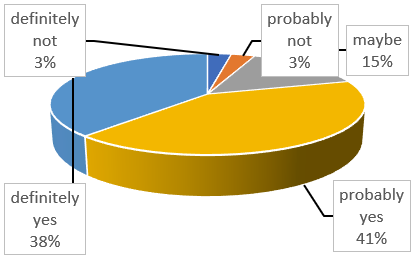
\includegraphics[width=\linewidth]{Imagens/Figure10.png}
    \caption{Recommending ChatGPT for academic use.}
    \label{fig-10}
    \source{Own elaboration (2024).}
    \end{minipage}
\end{figure}

The central tendency was to choose ``probably yes" (Mdn=4), and respondents mostly agreed with each other (IQR=1) (Table \ref{fig-6}).

%---- CÓDIGO DA TABELA 6 ----%
\begin{table}[h!]
\centering
\caption{Future recommendations of respondents.}\label{tab-6}
\begin{tabularx}{\textwidth}{@{}Xccccc cc@{}}
\toprule
Question & Definitely not & Probably not & Maybe & Probably yes & Definitely yes & Mdn & IQR \\
\midrule
Would you recommend ChatGPT? & 1 (3\%) & 1 (3\%) & 5 (15\%) & 14 (41\%) & 13 (38\%) & 4 & 1 \\
\bottomrule
\end{tabularx}
\source{Own elaboration (2024).}
\end{table}


According to previous research, sixty percent of teachers strongly recommended using ChatGPT in teaching writing, thirty percent were unsure and ten percent were negative because of plagiarism concerns \cite[p. 331-332]{nguyen2023}.

ESL teachers’ feedback on additional features for ChatGPT contributes to the ongoing evolution of the tool to meet the needs of language educators. Completing the survey in our research, some ESL teachers shared that they would like ChatGPT to have ``an additional feature of checking the uniqueness of a piece of writing", to offer ``a wider range of tasks", to assist ``during the revision and editing stages", ``create more sophisticated tasks", and ``compile tests and assessment". Some comments were rhetorical: ``AI cannot replace humans"; some humorous: ``to make it conduct lessons instead of me"; some skeptical: ``from the perspective of programming it may not be feasible"; and some critical: ``People are lazy! They have to think and be creative!". Similar to ESL teachers’ remarks on the necessity to learn how to receive high-quality responses from ChatGPT, some studies explore the patterns of creating effective prompts \cite{herfteducator2023, kim2023, kostka2023}.

Providing additional comments, respondents characterized ChatGPT as ``a huge gift for teachers", ``a wonderful work assistant", ``a great help for teachers if used properly and moderately". ESL teachers wrote about a positive effect on their lives, describing ChatGPT: ``It’s a great time-saver, I don’t feel like a robot anymore as I can focus on more creative tasks". Participants of another study had similar attitudes, mentioning that ChatGPT reduced their workload \cite[p. 38]{nguyen2023}. Previous research confirmed the effectiveness of ChatGPT in designing ESL courses \cite[p. 85]{kim2023}.

Some teachers acknowledged the necessity of professional development: ``I need more seminars, manuals on how to communicate with chat". There are similarities with previous research, which emphasized the importance of professional training on ChatGPT incorporation into language teaching \cite[p. 19]{nguyen2023}. Chinese ESL university teachers in another study expressed their concern over their insufficient technology use and expressed the need to increase their intrinsic motivation to improve their practices, which confirmed the necessity to facilitate ESL teachers by ensuring technology support and professional development programs \cite[p. 83]{huang2019}. According to the findings of another study on technology integration into ESL, there are four barriers, three of which are related to teachers and one to students. The most serious challenges for teachers were time constraints to implement technology-integrated lessons, low levels of IT competency and no technical support \cite[p. 30]{hsu2016}.

\section{Limitations and further research}
The limitation of this study lies in the fact that it collected data from university teachers working in Ukraine during wartime, therefore presenting the views and experiences of one particular category of educators. This exploratory study requires further research, which could investigate perceptions of educators with wider levels of expertise and areas of professional interest.

\section{Conclusion}
The paper aimed to explore ESL teachers’ attitudes and experiences using ChatGPT. Respondents were represented by university lecturers who were mostly middle-aged women, with experience of teaching English for about twenty years or more. According to the research results, most respondents used ChatGPT occasionally, mainly to prepare writing assignments for students, write articles and textbooks, or understand complex concepts. Nearly sixty percent of ESL teachers claimed that they were satisfied with ChatGPT’s assistance, and a quarter of respondents seemed to be indifferent. Whereas the participants were positive but cautious in assessing ChatGPT’s impact on teaching, rating it as moderate, half of them thought it positively influenced their performance as ESL teachers. Regarding how user-friendly ChatGPT was for respondents, it was easy or very easy for two-thirds of university teachers. However, more than half of them described challenges or limitations they experienced, listing faulty or irrelevant information that needed checking, low-quality responses and ethical issues. Interestingly, the majority of ESL teachers would recommend implementing ChatGPT in teaching. Whereas it saves time for teachers doing routine tasks, providing immediate feedback and generating ideas, it is evident that ESL teachers need more training and support aimed at developing AI literacy. ChatGPT’s integration by university teachers should include its creative use, getting feedback from students, monitoring their academic performance, reflecting on their experience, and being aware of its drawbacks. Further research needs to be carried out to investigate perceptions of educators with wider levels of expertise and areas of professional interest and university students’ experiences.


\printbibliography\label{sec-bib}
% if the text is not in Portuguese, it might be necessary to use the code below instead to print the correct ABNT abbreviations [s.n.], [s.l.]
%\begin{portuguese}
%\printbibliography[title={Bibliography}]
%\end{portuguese}


%full list: conceptualization,datacuration,formalanalysis,funding,investigation,methodology,projadm,resources,software,supervision,validation,visualization,writing,review
\begin{contributors}[sec-contributors]
\authorcontribution{Oksana Chugai}[datacuration,formalanalysis,investigation]
\authorcontribution{Iryna Lytovchenko}[methodology,validation]
\authorcontribution{Oksana Synekop}
[review,visualization]
\end{contributors}

\end{document}

